\documentclass{article}
\usepackage[ngerman]{babel}
\usepackage[T1]{fontenc}
\usepackage[utf8x]{inputenc}
\usepackage{graphicx}
\usepackage{spreadtab}
\usepackage{booktabs}
%\usepackage{hyperref}
\usepackage[left=25mm,right=25mm,top=20mm,bottom=20mm]{geometry}
\usepackage{siunitx}

\title{Pflichtenheft}
\date{\today}
\author{Projekt 3 EIT, Team 2: Reto Freivogel, Alexander Murray, Raphael Frey}

\begin{document}
\maketitle

\section{L\"osungskonzept}
\begin{figure}[h!]
    \begin{centering}
    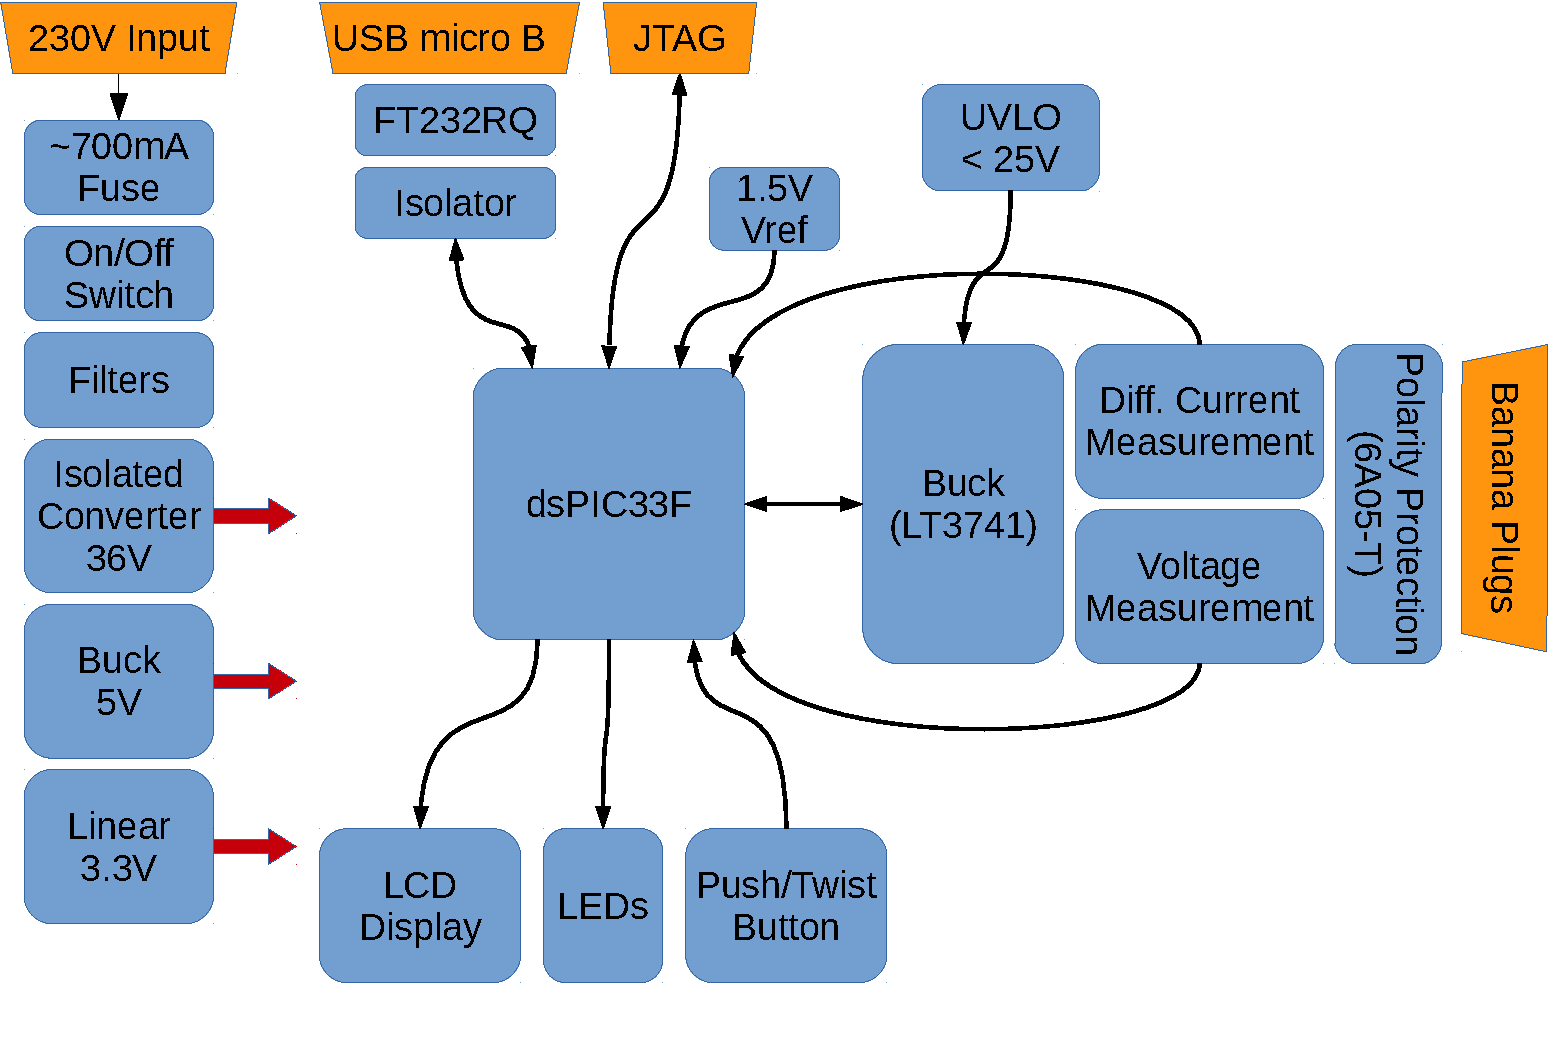
\includegraphics[width=.667\textwidth]{grob-blockdiagramm.pdf}
    \caption{Blockdiagramm des L\"osungsansatzes}
    \end{centering}
    \label{fig:grob-blockschaltbild}
\end{figure}

Das Kernst\"uck des Ger\"ates besteht  aus dem CVCC (Constant Voltage Constant
Current) Spannungswandler  und dem Mikrocontroller. Der  Mikrocontroller misst
differentiell  Ausgangsstrom und  Single-Ended Ausgangsspannung  anhand seiner
eingebauten  $ADC$s  und kann  somit  durch  zwei  $DAC$s die  Spannungs-  und
Stromlimite  des Wandlers  regeln. Damit  bildet er  die  I-V Kennlinie  eines
PV-Moduls nach.

Neben  den  Ausgangsspannungs-  und Ausgangsstromanforderungen  und  dynamisch
einstellbarer   Strombegrenzung  ist   eine   der  wichtigsten   Eigenschaften
des  Spannungswandlers  die  F\"ahigkeit,  Strom  aufnehmen  zu  k\"onnen  bei
Serieschaltung des  Ger\"ates mit anderen Simulatoren.   Der verwendete LT3741
von \emph{Linear} erf\"ullt alle diesbez\"uglichen Anforderungen.

Der LT3741  arbeitet mit Steuerspannungen  im Bereich von  $\SI{0}{\volt}$ bis
$\SI{1.5}{\volt}$. Damit die  h\"ochstm\"oglichste Aufl\"osung der  $ADC$s und
$DAC$s erzielt  werden kann, wird eine  Referenzspannung von $\SI{1.5}{\volt}$
(siehe Abbildung \ref{fig:grob-blockschaltbild}) verwendet.

Die  Ausgangsspannung ist  mit Hilfe  einer Diode  verpolungsgesch\"utzt.  Die
Kennlinie der Solarzelle geht somit nicht  ins Negative, sondern flacht bei 0V
ab.

Der   LT3741  kann   per  Software   ein-  oder   ausgeschalten  werden,   und
wird  zus\"atzlich   (mit  Vorrang)   in  Hardware  ausgeschaltet   falls  die
$\SI{36}{\volt}$-Speisung unter ca. $\SI{25}{\volt}$  f\"allt. Das erlaubt ein
kontrolliertes  und Vorhersehbares  Verhalten des  Spannungswandlers w\"ahrend
Ein- und Ausschaltvorg\"angen des Endproduktes.

Die Solarzelle wird mit folgender Formel modelliert:
\begin{equation}
I_d = I_{sc} \cdot \left(\frac{G}{G_0} - exp\left(\frac{V_d-V_{oc}}{V_t}\right)\right)
\end{equation}

Wobei   $I_{d}$   der   momentane  Strom,   $I_{sc}$   der   Kurzschlussstrom,
$\frac{G}{G_0}$    das   Beleuchtungsverh\"altnis,    $V_d$   die    momentane
Ausgangsspannung, $V_{oc}$  die Leerlaufspannung und $V_t$  die Dunkelspannung
aller Zellen in Serie sind. Der Einfluss der Temperatur wird in dieser Formel
vernachl\"assigt (nur relevant falls $V_{oc} > 5 \cdot V_t$).

Das   Ger\"at  wird   \"uber  ein   Text-LCD  und   einen  Dreh-Dr\"uck-Taster
bedient. Weiter  ist  ein  Ein-Aus  Schalter vorgesehen. Auf  dem  LCD  werden
die  Momentanwerte  der  Spannung  und  des  Stromes  sowie  die  eingestellte
Belechtungsst\"arke   angezeigt. Bei   Drehung   des  Drehtasters   wird   die
Beleuchtungsst\"arke ver\"andert. Durch  Dr\"ucken des Tasters gelangt  man in
Untermen\"us,  in denen  man  die anderen  Parameter  ($I_{sc}$, $V_{oc}$  und
$V_t$) ver\"andern kann.

Es  wird  ein  galvanisch  getrennter  USB  micro  B  Anschluss  eingebaut, um
Kommunikation mit einem externen Ger\"at zu erlauben. Zum Debuggen des Systems
wird diese Funktionalit\"at sehr n\"utzlich sein.


\section{Ziel-Spezifikationen}
\begin{center}
\begin{tabular}{lr}
    Maximale Ausgangsspannung	& 24V    \\
    Maximaler Ausgangsstrom		& 3.5A   \\
    Effizienz bei Volllast		& 80\%   \\
    Leistungsverbrauch Leerlauf	& 3W     \\
    Nachregelzeit				& 1ms    \\
    Genauikeit Spannung			& 2\%    \\
    Genauikeit Strom			& 2\%    \\
    Rippel Spannung				& 300mV  \\
    Rippel Strom				& 100mA  \\
    Stufen Kennlinie			& 3      \\
\end{tabular}
\end{center}


\section{Kostensch\"atzung}

Die wichtigsten Komponenten sind in der folgenden Tabelle aufgelistet.

\begin{center}
\begin{spreadtab}{{tabular}{lrrr}}
    \toprule
    @ Beschreibung & @ Preis & @ Anzahl & @ Betrag \\
    \midrule
    % Logik
    @ dsPIC33 microcontroller         & 4.91  & 1 & [-2,0] * [-1,0] \\
    @ ADuM5241 (Digital Isolator)     & 6.96  & 1 & [-2,0] * [-1,0] \\
    @ FT232RQ (UART to serial)        & 4.5   & 1 & [-2,0] * [-1,0] \\
    @ LCD Display, 80 (4x20) chars    & 27    & 1 & [-2,0] * [-1,0] \\
    @ Twist/Pushbutton                & 4.21  & 1 & [-2,0] * [-1,0] \\
    @ \SThiderow                      & @     & @ & sum(d2:d6)      \\
    % Schaltregler
    @ CVCC buck converter             & 8.44  & 1 & [-2,0] * [-1,0] \\
    @ MOSFET                          & 5     & 2 & [-2,0] * [-1,0] \\
    @ \SThiderow                      & @     & @ & sum(d8:d9)     \\
    % Speisungen
    @ ACDC 230V to 36V supply module  & 27.41 & 1 & [-2,0] * [-1,0] \\
    @ Power entry connector           & 15.96 & 1 & [-2,0] * [-1,0] \\
    @ LT3973 (36V to 5V buck)         & 5.88  & 1 & [-2,0] * [-1,0] \\
    @ \SThiderow                      & @     & @ & sum(d11:d13)    \\
    % Misc
    @ Housing                         & 26.92 & 1 & [-2,0] * [-1,0] \\
    @ Misc. components                & 75    & 1 & [-2,0] * [-1,0] \\
    @ Printed Circuit Board           & 40    & 1 & [-2,0] * [-1,0] \\
    @ \SThiderow                      & @     & @ & sum(d15:d17)    \\
    \\
    \midrule
    @ \textbf{Total}                  & @     & @ & d7+d10+14+d18   \\
    \bottomrule
\end{spreadtab}
\end{center}

\section{Testkonzept}

\begin{itemize}
    \item
        Testen der oben angegebenen Spezifikationen.
    \item
        Verhalten  von  Strom  und   Spannung  bei  verschiedenen  resistiven,
        kapazitiven und induktiven Lasten (und Kombinationen davon).
    \item
        Verhalten von  Floating Potential und Stromaufnahme  bei verschiedenen
        resistiven,  kapazitiven  und  induktiven  Lasten  (und  Kombinationen
        davon).
    \item
        Verifikation  der korrekten  Funktionsweise  des Interfaces  (Display,
        Drehknopf).
\end{itemize}
\end{document}
